\documentclass[a4paper,10pt]{article}
\usepackage{amsmath}
\usepackage{amssymb}
\usepackage[polish]{babel}
\usepackage{polski}
\usepackage[utf8]{inputenc}
\usepackage{indentfirst}
\usepackage{geometry}
\usepackage{array}
\usepackage[pdftex]{color,graphicx}
\usepackage{subfigure}
\usepackage{afterpage}
\usepackage{setspace}
\usepackage{color}
\usepackage{wrapfig}
\usepackage{listings}
\usepackage{datetime}

\renewcommand{\onehalfspacing}{\setstretch{1.6}}

\geometry{tmargin=2.5cm,bmargin=2.5cm,lmargin=2.5cm,rmargin=2.5cm}
\setlength{\parindent}{1cm}
\setlength{\parskip}{0mm}

\newenvironment{lista}{
\begin{itemize}
  \setlength{\itemsep}{1pt}
  \setlength{\parskip}{0pt}
  \setlength{\parsep}{0pt}
}{\end{itemize}}

\newcommand{\linia}{\rule{\linewidth}{0.4mm}}

\definecolor{lbcolor}{rgb}{0.95,0.95,0.95}
\lstset{
    backgroundcolor=\color{lbcolor},
    tabsize=4,
  language=C++,
  captionpos=b,
  tabsize=3,
  frame=lines,
  numbers=left,
  numberstyle=\tiny,
  numbersep=5pt,
  breaklines=true,
  showstringspaces=false,
  basicstyle=\footnotesize,
  identifierstyle=\color{magenta},
  keywordstyle=\color[rgb]{0,0,1},
  commentstyle=\color{Darkgreen},
  stringstyle=\color{red}
  }

\begin{document}

\noindent
\begin{tabular}{|c|p{11cm}|c|} \hline 
Z2 & Przemysław Kleszcz, Krzysztof Tatar & \ddmmyyyydate\today \tabularnewline
\hline 
\end{tabular}


\section*{Zadanie 1 - Rozmycie Gaussa w OpenMP}

Celem zadania było napisanie programu, który rozmywa zadane zdjęcie za pomocą algorytmu Gaussa z maską o wymiarach 5x5. Do poprawnego działania programu należy podać trzy argumenty wejściowe. Są to \emph{n -liczba wątków}, \emph{input\_image - ścieżka do pliku obrazu w formacie JPEG} i \emph{output\_image - ścieżka do pliku wyjściowego obrazu w formacie JPEG
}.Poniżej przedstawiony jest rysunek zastosowanej filtracja na podstawie filtra o masce 5 x 5 wraz z wagami, które są wykorzystywane podczas przeprowadzania obliczeń.

\begin{figure}[!ht]
	\centering
 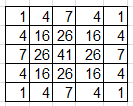
\includegraphics[width=0.2\textwidth]{3.png}
  \caption{Wykorzystana maska Gaussowska}
\end{figure}

Poniżej zaprezentowano główną funkcję programu odpowiedzialną za zrównoleglanie obliczeń.

\begin{lstlisting}
void gaussian(int weight,Mat picture,Mat pictureNew,int kernel[][5],int threadsNumber)
{
	int y, x;
	int r, g, b;

#pragma omp parallel shared(picture,pictureNew) num_threads(threadsNumber) private(r,g,b,y,x)
	{
#pragma omp for schedule(guided,1)
		for (y = 0; y < picture.rows; y++)
		{
			for (x = 0; x < picture.cols; x++)
			{
			...
			...
			...
			}
		}
	}
}
\end{lstlisting}

W powyższym programie został zastosowany algorytm filtrowania za pomocą którego posiadamy możliwość rozmycia podanego obrazka. Do zrównoleglenia głównej pętli for została użyta dyrektywa OpenMP.Wyraz omp jest słowem kluczowym biblioteki. Dyrektywa parallel, wskazuje kompilatorowi obszar kodu,
który  będzie  zrównoleglony.
\newline
\newline
Zrównoleglenie głównej pętli for: 
\begin{lstlisting}
#pragma omp for
\end{lstlisting}
 Kolejna dyrektywa - for - informuje kompilator, że zrównoleglana będzie pętla typu for.
\newline
\newline
Określnie, które zmienne będą wspólne shared, a które prywatne private:
\begin{lstlisting}
shared(picture,pictureNew) private(r,g,b,y,x) 
\end{lstlisting}
Zmienne wspólne są dostępne dla każdego wątku, natomiast do danej zmiennej prywatnej ma dostęp tylko jeden określony wątek. W naszym programie zmiennymi prywatnymi są: r,g,b,y,x, a zmiennymi wspólnymi picture,pictureNew.
\newline
\newline
Dyrektywa schedule: 
\begin{lstlisting}
schedule(guided, 1)
\end{lstlisting}
Za pomocą polecenia schedule możemy kontrolować sposób w jaki OpenMP przydziela iteracje dostępnym wątkom. Parametr guided powoduje przypisanie do każdego wąktu odpowiednio dużego fragmentu następujących po sobie iteracji. Rozmiar fragmentu zmniejsza się wykładniczo, wraz z każdym pomyślnym przypisaniem, do minimalnego rozmiaru zdefiniowanego w parametrze „chunk”. Parametr „chunk” jest ustawiony na 1, oznacza to że rozmiar każdego z początkowych zbiorów jest opisany wyrażeniem:
\begin{center}liczba\_nieprzydzielonych\_iteracji/liczba\_wątków
\end{center}
Dyrektywa num\_threads: 
\begin{lstlisting}
num_threads(threadsNumber)
\end{lstlisting}
Za pomocą dyrektywy num\_threads określamy, ile wątków ma być użytych do zrównoleglenia pętli for.
\newline
\newline

\begin{figure}[!ht]
	\centering
 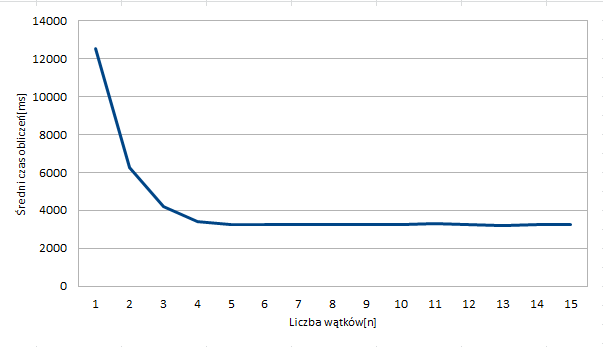
\includegraphics[width=0.7\textwidth]{1.png}
  \caption{Wykres średniego czasu obliczeń}
\end{figure}

Z powyższego rysunku można wywniokoswać, że średni czas obliczeń dynamicznie malał dla pierwszych 4 wątków. Następnie dla kolejnych wątków średni czas jest ustabilizowany.
Poniższy rysunek jest dobrym przykładem opisanego zjawiska.

\begin{figure}[ht]
	\centering
  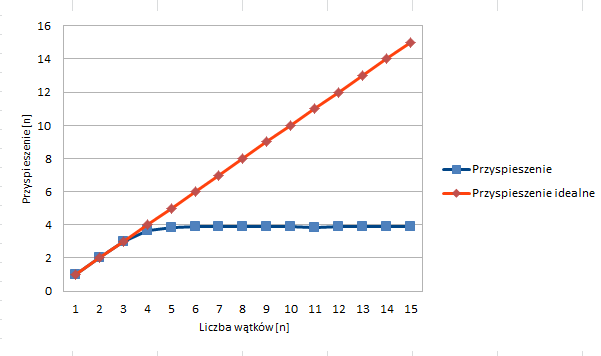
\includegraphics[width=0.7\textwidth]{2.png}
  \caption{Wykres przyspieszenia}
\end{figure}

Powyższe zadanie zostało zrównoleglone dzięki bibliotece OpenMP. Dzięki zastosowaniu dyrektyw biblioteki udało się uzyskać czterokrotne przyspieszenie dla 4 wątków. Dla kolejnych 11 wątków, w tym przykładzie nie wpłynęły znacząco na wydajność.


\end{document}
